\chapter{Numerical solution of optimal avoidance for PM}\label{cha:ch4}
To determine the numerical solution of optimal avoidance for PM, the following OCP is formulated:
\begin{align}
    & \underset{F_x,\ F_y}{\text{Min}}
    & & & \mu\\
%
    & \text{subject to} 
    & & & F_x &\leq 0 & 0 &\leq F_y & F_x^2 + F_y^2 &\leq F_{\text{max}}^2,\\
%
    &&& & \dot x &= v_x, & \dot y &= v_y, & \dot v_x &= \frac{F_x}{m}, & \dot v_y &= \frac{F_y}{m},\\
%
    &&& & x(t_o) &= 0, & y(t_o) &= 0, & v_x(t_o) &= v_o, & v_y(t_o) &= 0,\\
    &&& & x(t_f) &= \text{A}+25, \\
    &&& & f_o(x,y) &>= 1 ,
\end{align}
where 
\begin{equation}
    f_o(x,y) = \left(\frac{x-\text{A}}{R_1}\right)^n + \left(\frac{y}{R_2}\right)^n
\end{equation}
is the obstacle, $F_{\text{max}} = \mu m g$, and the vehicle parameters are presented in Table~\ref{tab:num_sol_opt_avoid_PM_params}.
\begin{table}[h!]
    \begin{subtable}{0.38\textwidth}
        \begin{tabular}{c|c}
            \multicolumn{2}{c}{Vehicle} \\
            \hline
            $m$ & 2000\,kg \\
            $g$ & 9.81\,m/s\textsuperscript{2} \\
            \multicolumn{2}{c}{Obstacle} \\
            \hline
            $R_1$ & 5 \\
            $R_2$ & 3 \\
            $n$ & 20 \\
        \end{tabular}
        \caption{Vehicle PM and obstacle parameters.}
        \label{tab:num_sol_opt_avoid_PM_params}
    \end{subtable}
    \hfill
    \begin{subtable}{0.58\textwidth}
        \begin{tabular}{c|c|c|c}
            & & Analytical & Simulation\\
            A & B & $\mu$ & $\mu$ \\
            % [m] & [-] & [m] & [-] \\
            \hline
            20.5047\,m & 2.9012\,m & 0.5546 & 0.5583
        \end{tabular}
        \caption{Numerical and analytical solutions for minimum road friction for optimal obstacle with $v_0 = 20$\,m/s.}
        \label{tab:num_sol_opt_avoid_PM_res}
    \end{subtable}
    \caption{Brake or evade for straight-line braking.} 
    \label{tab:num_sol_opt_avoid_PM}
\end{table}

\section{Analytical solution}
The analytical solution is determined by first calculating $\gamma$, 
\begin{align}
    \gamma &= \arctan\left(\frac{\text{B}}{\text{A}}\right),
\end{align}
where B and A are the height and distance of the obstacle and the trajectory intersection point, assuming that the vehicle is starting from (0,0). 
$\theta$ is calculated using the relation
\begin{align}
    \theta &= \frac{\gamma + \arcsin\left(3\sin\left(\gamma\right)\right)}{2}.
\end{align}
Now, $\mu$ is calculated using 
\begin{align}
    \mu &= \frac{2\sin\left(2\gamma\right)\cos\left(\theta\right)}{\cos\left(\theta-\gamma\right)^2}\frac{v_o^2}{2g\text{A}}.
\end{align}
The comparison between the optimal and analytically calculated $\mu$ is presented in Table~\ref{tab:num_sol_opt_avoid_PM_res}.

\subsection{Code}
The source codes for this problem can be found at \newline \href{https://github.com/arvba41/optimal_vehicle_maneuvers/blob/main/uppgift/ugf4/opti_veh_men_prt.m}{https://github.com/arvba41/optimal\_vehicle\_maneuvers}.

The detailed results of the optimization problem are presented in Figure~\ref{fig:num_sol_opt_avoid_PM_res_pic}.
\begin{figure}[h!]
    \centering
    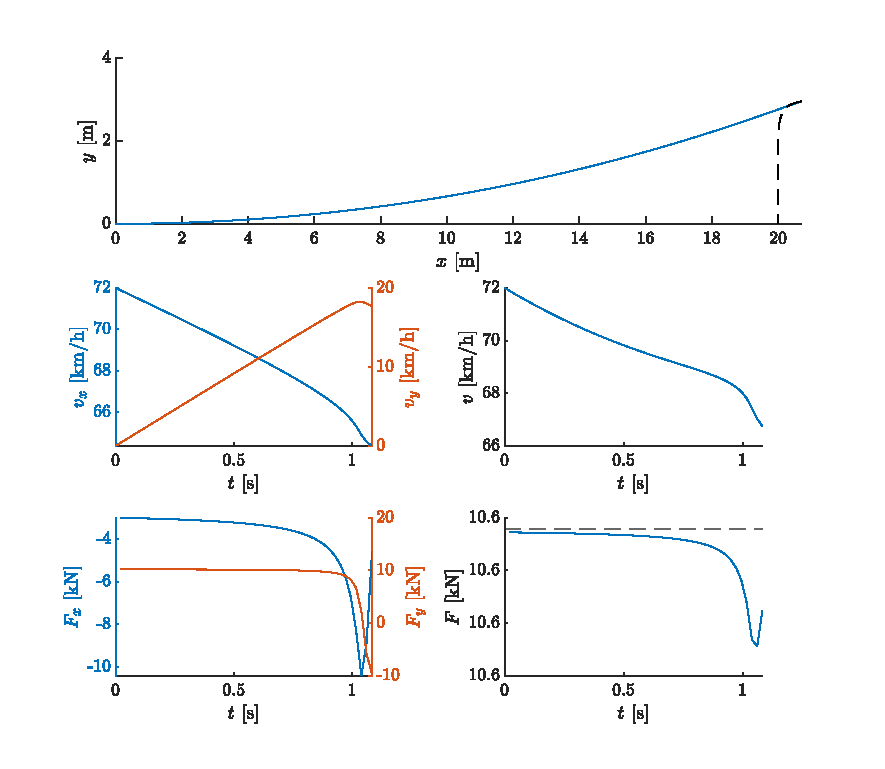
\includegraphics{figures/prob4_opt_avoid_path.pdf}
    \caption{Numerical solution for the optimal obstacle avoidance.}
    \label{fig:num_sol_opt_avoid_PM_res_pic}
\end{figure}
